\documentclass{bioinfo}
\copyrightyear{2005}
\pubyear{2005}

\usepackage[hyphens]{url}
\usepackage[square,numbers]{natbib}

\begin{document}
\firstpage{1}

	
\newcommand{\OnePhaseone}{phase1\_chr1}
\newcommand{\NinteenPhaseone}{phase1\_chr19}
\newcommand{\SevenPhaseone}{phase1\_chr1-7}
\newcommand{\FullPhaseone}{phase1\_chr1-22}
\newcommand{\OnePhasethree}{phase3\_chr1}
\newcommand{\ThreePhasethree}{phase3\_chr1-3}
\newcommand{\FullPhasethree}{phase3\_chr1-22}
\newcommand{\ARI}{Adjusted Rand Index}

\title[MapReduce Clustering]{Scalable Clustering of Genotype Information using MapReduce}
\author[O'Brien \textit{et~al}]{Aidan R. O'Brien\,$^{1,2}$, Neil Saunders\,$^1$,Fabian A. Buske\,$^{3,4}$ and Denis C. Bauer\,$^1$\footnote{to whom correspondence should be addressed}}
\address{$^{1}$CSIRO, Digital Productivity Flagship, 11 Julius Av, 2113, Sydney, Australia\\
$^{2}$School of Biomedical Sciences and Pharmacy, Faculty of Health, 2308 Newcastle, Australia\\
$^{3}$Cancer Epigenetics Program, Cancer Research Division, Kinghorn Cancer Centre, Garvan Institute of Medical Research, 384 Victoria St, 2010, Sydney, Australia\\
$^{4}$UNSW Medicine, University of New South Wales, 2052 Sydney, Australia.}

\history{Received on XXXXX; revised on XXXXX; accepted on XXXXX}

\editor{Associate Editor: XXXXXXX}

\maketitle

\begin{abstract}

\section{Motivation:}
Processing genomic information from whole genome sequence studies poses computational challenges due to the unprecedented data volume, which render transitional approaches insufficient. 
However, advancements in modern hardware accelerators and data processing provides the means for overcoming these limitations, with Hadoop the most popular approach.  
Here we compare implementation and resource consumption when clustering genome-wide variants using R as well as the Hadoop-based library, Mahout. To do this, we developed an interface between Mahout and the standard variant format (VCF), which opens up the use of advanced, efficient machine learning algorithms to genomic data. 
\section{Results:}
We achieve more than 2-fold speedup by using the scalable k-means MapReduce implementation over the equivalent analysis performed in R, by comparable accuracy. However, the real advantage lies in the scalability of MapReduce beyond R's capability to a genome-wide analysis. We successfully clustered more than 2,500 individuals each having more than 81 Million variants. 
\section{Availability:}
The package is written in Java and available at \url{https://github.com/BauerLab/GeMaIn}.

\section{Contact:} \href{Denis.Bauer@CSIRO.au}{Denis.Bauer@CSIRO.au}
\end{abstract}

\section{Author CV}
\paragraph{Aidan R O'Brien, BBiot(Hons), is a joined researcher at Newcastle University and CSIRO and interested in BigData approaches for pan-cancer research.}

\paragraph{Neil Saunders, PhD, is a research scientist at CSIRO interested in systems biology approaches for human health.}

\paragraph{Fabian A. Buske, PhD, is a computer science expert focusing on no-SQL database systems.}

\paragraph{Denis C Bauer, PhD, is team leader of the transformational bioinformatics team at CSIRO active in the personalised genomics space.}


\section{Introduction}

Grouping individuals based on their genomic profile is a commonly performed tasks to identify population structure~\citep{Gao2007} or elucidate different haplotype involvement in diseases susceptibility~\citep{Laitman2013}.  
Traditionally both, the number of individuals and included genotypes (typically from SNP arrays), were relatively small and libraries in Bioconductor, which commonly perform all calculations in memory, sufficient. 
However, recent technological advances in whole genome sequencing have made population-scale sequencing feasible. 
It is hence economical to generate studies with sample sizes previously reserved for larger consortia such as the 1000 genomes project~\citep{1KG2012} or The Cancer Genome Atlas, TCGA~\citep{TCGA2013}. 
At the same time, whole genome sequencing enables the inclusion of rare or even somatic mutations in the analysis, increasing the feature space by orders of magnitude. This drastic increase in both sample numbers and features per sample requires a massively parallel approach to data processing. 

As a result of these big data challenges, MapReduce approaches are increasingly being used in bioinformatics (for reviews see~\citep{Zou2013, Qiu2010,Taylor2010}). This is especially the case for sequence analysis tasks, such as read mapping~\citep{Schatz2009}, duplicate removal~\citep{Jourdren2012}, and variant calling~\citep{Langmead2009, McKenna2010} as well as Genome Wide Analysis Study based tasks~\citep{Huang2013, Guo2014}.

At the same time, computer scientists extent MapReduce paradigms to cope with the iterative nature of machine learning tasks~\citep{Chu2009}. Specifically, the Mahout project \url{https://mahout.apache.org/} has been developed extensively~\citep{Ranger2007, Owen2011} and was successfully applied in the clinical informatics space~\citep{Dong2013}.

In this paper, we link the two areas of parallel machine learning and bioinformatics by providing an interface between Mahout and the standard variant data format, variant call format (VCF)~\citep{1KG2012}, which opens up the application of Mahout's different machine learning algorithms to be applied to genotype-based tasks. 
To demonstrate the capability, we cluster variant datasets from the 1000 genomes project to determine population structure using the k-means clustering algorithm available in Mahout. In the first section we benchmark the performance and accuracy of Mahout's implementations against a standard R based implementation on a subset of the data and in following two sections we investigate Mahout's scaleability with respect to sample size and features per sample. We then discuss design considerations for the resource allocation and give a visualisation example in the last two sections.  

\section*{Results and discussion}

% COMPARISON TO R
\subsection*{Clustering in Mahout requires less memory than in R}
In this section, we compare the runtime and resource requirements between the k-means clustering implementation in R and Mahout for the small \NinteenPhaseone{} dataset (see Methods, Table~\ref{Tab:01}). 
We measured the runtime separately for pre-processing stage as well as the clustering stage. 

With Hadoop, pre-processing the data takes approximately 6 minutes, with an allocation of up to 3GB memory. 
The resulting data is stored as a Hadoop 'SequenceFile' of about 835MB in size.
Conversely,  pre-processing the data to R's in-memory matrix takes 56 minutes and required 17.7GB memory. 
K-means clustering the data, however, is faster with R, using 7s, whereas Mahout takes just under 9 minutes (see Table~\ref{Tab:02}). 
This is due to the additional overhead involved in spawning the map and reduce processes, and distributing the data between nodes.
R, on the other hand, already has the entire matrix in-memory, on a single machine and since no disk-access or networking is required the clustering can be performed faster. 
Due to the relatively small number of variants, cluster accuracy is relatively poor for both methods, with the best \ARI{}~\citep{Hubert1985} score for clustering individuals in one of 4 populations (see Methods) being 0.705 in Mahout and 0.614 in R (see Table~\ref{Tab:02}, an \ARI{} of 1 means perfect clustering).

While the overall processing time is 40 minutes faster in Mahout compared to R, the real bottleneck for large datasets is the amount of memory available on a single machine. 
As an example, the entire set of 1000 Genomes Project phase3 variants could require approximately 1.6TB to be completely loaded into memory as a double-precision matrix (see Table~\ref{Tab:01}). This is based on the equation:
$\frac{n \times m \times 8\text{bytes}}{1\text{GB}}$, where $n \times m$ are the matrix dimensions, 8bytes is the memory a \texttt{double} occupies (i.e. each matrix element), and  1GB is $10^9$ bytes.

Therefore, the data processed in the subsequent sections are too large to be processed with standard R, hence we focus on evaluating different settings of the Mahout implementation only.  



% (1) SCALING UP FEATURES IN MAHOUT
\subsection*{Hadoop scales to genome-wide clustering}
In this section we demonstrate Mahout's ability to cluster genome-wide variants. 
To demonstrate accuracy-gain and resource-consumption we evaluate whole-genome data (\FullPhasethree{}), which contains 79 million variants, as well as two subsets with 19 (\ThreePhasethree{}) and 6 million (\OnePhasethree{}) variants, respectively  (see Table~\ref{Tab:01}).  
As expected, providing variants from only chromosome one (\OnePhasethree{}) holds to little information and hence achieves a relatively low \ARI{} of 0.622 (see Table~\ref{Tab:02}).
Note, phase3 data has one more population group, which explains the decrease in accuracy compared to the previous section.  

Increasing the input to include the first three chromosomes (\ThreePhasethree{}) improves the accuracy with an \ARI{} of 0.825 (Table~\ref{Tab:02}).
We are reaching a saturation point for k-means clustering here, as including all 22 autosomes (\FullPhasethree{}) improves the \ARI{} only marginally to 0.84 (Table~\ref{Tab:02}).
However, this demonstrates that performing clustering using whole-genome variants on research infrastructure using Mahout is feasible as the resource consumption lies within realistic boundaries. 
The time consumption increases to 25 hours and memory to 6 GB (Table~\ref{Tab:02}). 


% (2) SCALING UP SAMPLES IN MAHOUT
\subsection*{Hadoop scales effortlessly to more than twice the number of samples}
Hadoop's main advantage over other parallelisation techniques is its ability to scale to more samples without altering the code. 
Mahout's k-means algorithm is structured such that it splits the clustering problem into separate, smaller tasks, where each task calculates the distance between a subset of samples and the k-means centroids. 
The scalability is achieved by Hadoop creating 'containers' for each task and subsequent iterative processing until every task is completed.
We discuss containers in greater detail in the next section, however, a container is essentially a pre-defined allocation of memory and CPU cores.
By increasing the number of samples, the k-means algorithm simply divides the job into more tasks, which enables the memory requirement of each task to stay the same.
This is because the dimensionality is constant, compared to the previous section where we increased the number of variants and observe a subsequent increase in memory. 

To demonstrate this, we compare k-means clustering of the 2504 individuals from the phase3 dataset compared to the 1092 individuals from the phase1 dataset.
We specifically use the \SevenPhaseone{} and \ThreePhasethree{} datasets because of their similar feature size.
The algorithm completed successfully with the same sized containers for both datasets, however, the \ThreePhasethree{} dataset required about twenty minutes more time than the smaller \SevenPhaseone{} dataset (Table~\ref{Tab:02}). 
This demonstrates Hadoop's strength of scaling with sample size. 


% (3) CLUSTER AND CONTAINER SIZE
\subsection*{Cluster size and containers}
In the previous section we observed that while the memory remained constant the runtime increases with sample size. 
On a larger Hadoop cluster the runtime could also stay constant if the number of additional tasks can be accommodated by additional compute nodes. 
However, as research is carried out on resource-finite infrastructure, we discuss in this section how to specify the optimal container size when designing MapReduce jobs to incur only a minimal increase in runtime. 

To elaborate, a container is essentially an abstraction of resources, i.e. memory and CPU cores. 
After Hadoop divides a job into tasks, each task runs in parallel in a container. Also, each container is independent of other containers.
The resources Hadoop allocates to each container is a predefined value, specified by the user in Hadoop's configuration. 
According to the Hortonworks documentation~\citep{Horton2013}, the general rule of thumb is that one CPU core is allocated to each container, and the available memory per node should be divided equally between each of those containers. 
For example, on a node with 8 CPU cores and 32GB memory, each container should be allocated 1 CPU core and 4GB memory. Effectively allowing a maximum of eight 4GB containers to run in parallel on that node.

When a MapReduce job is launched, Hadoop spawns a number of map tasks and reduce tasks. 
These tasks are placed in a queue until a node has enough resources available to run a container, and generally, the more containers that can run simultaneously, the faster the job will complete.
For smaller jobs, the maximum number of containers are generally limited by the available CPU cores because each container requires an entire CPU core. The tasks running in each container may not be able to utilise all of the memory allocated to that container.
However, for jobs that deal with large datasets, the memory allocated per container (following Cloudera's guidelines) may not be enough.
We could modify the above example to allocate each container 1 CPU core and 8GB memory, however now only four containers can fit within the node's 32GB memory, resulting in the other 4 CPU cores being idle (as only four containers can run simultaneously). 
It is therefore optimal to allocate the appropriate resources to containers, and only increase container memory when necessary, as overallocation of memory will simply limit the number of simultaneous containers each node can run.

To demonstrate the importance of specifying these parameters correctly, we ran identical jobs, using different Hadoop configurations. 
The \OnePhaseone{} dataset only requires 1.5GB memory per container, as we demonstrated previously.
Increasing the map container size to 4GB results in the job taking an additional 5 minutes (see Table~\ref{Tab:03}), because fewer tasks can run in parallel. 
Attempting to run the larger data set (\FullPhasethree{}) with either 1.5GB or 4GB will result in the job failing, because the feature vectors do not fit into the available memory. 
At least 6GB memory per container and 21h runtime are required to finish the job. 

One of the main selling points of Hadoop, is that it will run on commodity hardware. 
To mimic the available resource in a standard resource setting we used only a small Virtual Machine cluster on Microsoft Azure for the benchmarking in this paper so far.
However, to demonstrate the scalability of Hadoop and our MapReduce algorithms, we also ran the clustering jobs on a much larger development Hadoop cluster. 
As presented in Table~\ref{Tab:03}, the \OnePhaseone{} job saw an improvement of approximately 70\% when providing 448 cores of 13GB. 
With these resources, the \FullPhasethree{} example, was 78\% faster.

Although both jobs were more than twice as fast on the larger cluster, the speed doesn't scale relative to the size of the cluster. This is due to a limitation in these examples, where the number of reduce tasks in k-means clustering is limited to the number of k-means clusters (k).
A task where k is five, for example, will only be able to spawn five reduce tasks, no matter how many resources are available. Although sometimes inevitable, this bottleneck of maximum simultaneous reduce tasks is an important consideration to take into account when designing MapReduce jobs. 

\begin{figure}[!tpb]%figure1
\centerline{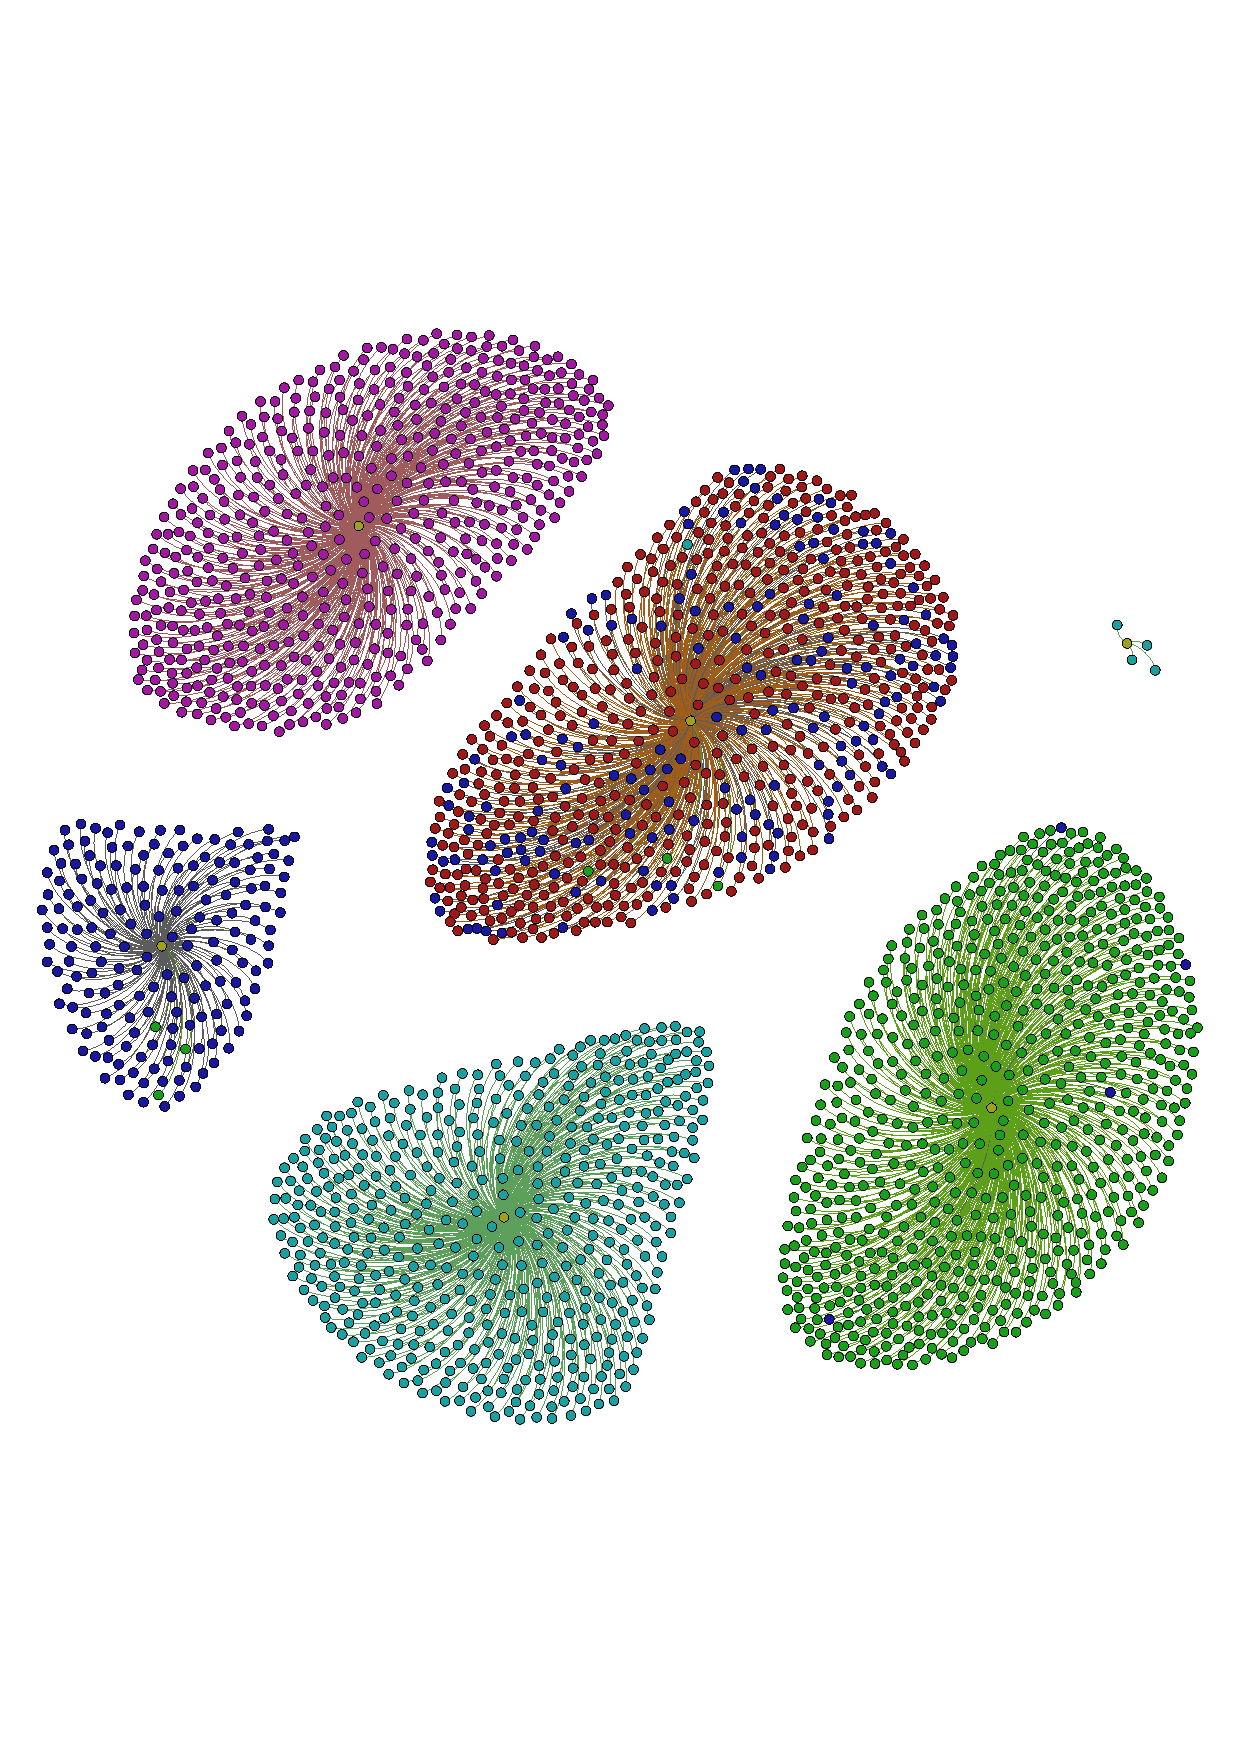
\includegraphics[type=pdf,ext=.pdf,read=.pdf, scale=0.40]{gephi-p3}}
        \label{fig:sign}
        \caption{{\bf Visualisation of k-means clusters derived from the phase 3 dataset.}
        Nodes are coloured by super population: AFR (green), AMR (blue), EAS (pink), EUR (red) and SAS (cyan). 
}
\end{figure}


\subsection*{Cluster visualisation}
GraphML files generated using Mahout Cluster Dumper can be visualised using popular freely-available tools such as Gephi~\citep{ICWSM09154}. An example visualisation using the \FullPhasethree{} dataset, with nodes coloured by super population, is shown in Figure 1.

The clusters generated by k-means clustering and their population structure are readily apparent. 
Three clusters are homogeneous, containing only East Asian (EAS, pink cluster) or South Asian (SAS) individuals (2 clusters, cyan cluster and the second small and unconnected).
Two clusters contain predominantly one super population plus a minor component of another: Ad Mixed American (AMR) + African (AFR) or AFR + AMR. 
The sixth cluster is predominantly a mix of European (EUR) + AMR, with 3 AFR individuals and 1 SAS.


\section*{Conclusion}
In this paper we have applied Mahout's k-means clustering to the task of clustering individuals, based on their genomic variants. 
We provide an interface from VCF format to Hadoop and Mahout, and a toolset to interpret Mahout's clustering output (see Figure 2).
Disregarding the pre-processing time, we find that on small datasets the clustering stage is two orders of magnitudes slower in Mahout compared to R (9 minutes vs 7 seconds), due to the overhead of setting up and co-ordinating the communication between the Hadoop nodes. 
However, increasing either the number of samples or the number of features per sample quickly exceeds the capability of R on the used machine due to memory limitations.
Hadoop on the other hand scales effortlessly to more than twice the number samples (2,504). It can also process VCF files that contain over 81 Million variants per samples, albeit with higher but still reasonable memory allocation (6G).
The MapReduce functions can scale from a relatively small and accessible cluster with 16 cores, to a much larger cluster with close to 500 CPU cores, although designing the container size for optimal resource and runtime consumption remains an expert task. 
In conclusion, Mahout offers a scalable out-of-the box solution that is directly applicable to genotype-based clustering for population or family association. 


\begin{methods}
\section{Methods}
\subsection*{Datasets}
We used variant call format (VCF) files from phases 1 and 3 of the 1000 Genomes Project.
Each VCF file details the genetic variation (SNPs and indels) for one chromosome, between each individual and a reference genome derived from GRCh37. 
The phase1 and phase3 datasets contain 1,092 and 2,504 individuals, respectively.
Metadata available from the 1000 Genomes Consortium specifies additional attributes for each individual, including population and familial data.\\
We used different subsets of the data for different comparisons. For example, to be able to compare Hadoop with R, we used the VCF file containing chromosome 19 variants (\NinteenPhaseone{}).
To demonstrate scaling with Hadoop, we use subsets that contain more variants, i.e. \SevenPhaseone{} and \FullPhaseone{}, which include chromosome 1-7 and the full genome, respectively.
Table~\ref{Tab:01} contains an overview of the datasets.

\subsection*{Hardware and Software}
We processed the data using a cluster of five VMs on the Microsoft Azure cloud service. Three of these VMs, the 'worker nodes', each have 14GB memory and and 8 CPU cores. These three VMs run the Hadoop2 NodeManager, which manages the Yet Another Resource Negotiator (YARN) 'containers' (see discussion).
The user is able to specify the resources allocated to each container, where map containers can have a different allocation to reduce containers.
The fourth VM runs the HDFS NameNode, ResourceManager and monitoring services, and the fifth VM, a small, single core machine, runs the Cloudera manager service.
With a total of 42GB memory and 24 CPU cores available between the node managers, we can simultaneously run up to 24 YARN containers with 1.5GB memory per container, or 12 YARN containers with 3GB memory per container.
Storage consists of a 3TB Hadoop Distributed File System (HDFS) partition distributed across the three worker nodes. Each of these nodes runs a DataNode with a 1TB disk.

The larger cluster mainly differs in regards to hardware. It has a total of 448 CPU cores and 1.31TB memory available. 

We used a single VM for the comparison between Mahout and R.

\subsection*{Pre-processing}
\label{Sec:preprocessing}
Mahout requires Hadoop's `SequenceFiles' as input to its machine learning algorithms. SequenceFiles are binary flat files consisting of key/value pairs. In this case, each of the keys is a
label for an individual, where the associated value for each key is a `sparse vector' representing the individual's genomic variants. We use sparse vectors, rather than
dense vectors, to significantly reduce required memory and disk space. Each sparse vector consists of two separate vectors. An item in the first vector is
effectively a key for an item at the same position in the second vector. The key represents a genomic location, where its value represents the variant. Zero values (positions where there is no variant)
are omitted. Therefore, the fewer variants in an individual's genome, the smaller the sparse vector size. In comparison, `dense vectors' are single arrays that
include every position where a variant may fall, whether or not there actually is a variant. Therefore, the size of a dense vector isn't reduced with a large number of non-variants.

The values of the sparse vectors, which, as previously mentioned, represent an individuals genomic variants, are a \texttt{double} java type.
We set the value of each double to the sum of the square root of the Hamming distance between each variant allele and the reference genome. Therefore, a value identical to the reference, 0\textbar{}0, will be 0 (and omitted from the sparse vector),
a heterozygous variant, 0\textbar{}1 or 1\textbar{}0, will be 1 (sqrt1) and a homozygous variant, 1\textbar{}1, will be 2 (sqrt1 + sqrt1). The square root of the each allele prevents variants such as 1\textbar{}1 colliding with the variant 2\textbar{}0.

We wrote two `MapReduce' classes in Java to convert VCF files to the aforementioned sequence files. This is scalable and should work on any number of files,
of any file size; limited only by disk space and time. 
The `map' stage of the first job parses each line of the VCF file to key value pairs. Each of the keys are an identical arbitrary number, where the value for each key is a sparse vector of the variants from each line. The variants in each vector are in the same order as they appear in the VCF file.

Additionally, in this stage, we can define parameters to exclude certain variants that may be deemed low quality, or only appear in a certain number of individuals.
We use identical keys so that each key value pair is sent to the same reducer, and this reducer assigns a unique key to each value. We require one reducer in this step to make each the key for each variant a consecutive number, rather than an arbitrary feature, such as its genomic location. Because keys are represented by integers, this helps to avoid integer overflows by keeping the keys relatively small.

The second job effectively transposes the output from the first job. The mappers create key value pairs where the key is a composite of the individual id and variant id, and the value is the variant.
This composite key, which is essentially a concatenation of two keys, allowed us to implement custom 'collect' and 'sort' classes to speed up the process. These classes divide up the key value pairs by their individual ID and sort them by their location ID, so each sorted collection of key/value pairs can be sent to a separate reducer.
 The reducers then write the variants for each individual to a sparse vector and stores each vector as a value, where the key is the individual ID.


\subsection*{Mahout K-means clustering}
To cluster the samples from the sequence files, we use Mahout 0.9 with Hadoop 2.5.0. 
The clustering steps are the same for each dataset, however, due to the increased feature size we designate more memory to the
YARN containers. For the first step, we specify \texttt{k}, the number of clusters. The function \texttt{RandomSeedGenerator.buildRandom} creates a new sequence file containing \texttt{k}
random centroids from the samples sequence file. The sequence file
of samples and the sequence file of centroids serve as the input to \texttt{KMeansDriver.run}, a static Mahout API function that launches
a k-means clustering job on the Hadoop service. 


\subsection*{R K-means clustering}
We use `readVcf' from the R library, `VariantAnnotation', to iteratively read in the VCF file. For each iteration, we convert the data to a matrix and
convert the values for each variant to a double, as mentioned previously. We then transpose the matrix, so individuals are represented
by rows, and append the matrix to that from the previous iteration. Once the matrix contains all of the variants from the VCF file, we cluster the data
using the `kmeans' algorithm from the `stats' library.



\subsection*{Clustering quality}
We scored the clusters with the \ARI{}~\citep{Hubert1985}. 
This index compares two different cluster sets, here the prediction $X = \{ X_1, X_2, \ldots , X_r \}$ and the annotated data $Y = \{ Y_1, Y_2, \ldots , Y_s \}$, and assigns a value based on the overlap between $X$ and $Y$ as captured in a contingency table $\left[n_{ij}\right]$ where each entry $n_{ij}$ denotes the number of objects in common between $X_i$ and $Y_j : n_{ij}=|X_i \cap Y_j|$. 
The \ARI{} is then 
{\tiny
\begin{eqnarray*}
ARI=\frac{\sum_{ij}{{n_{ij}\choose 2}} - \left[ \sum_{i}{{a_i\choose2}} \sum_{j}{{b_i\choose2}} \right] / {n\choose2}}{\frac{1}{2} \left[ \sum_{i}{{a_{i}\choose 2} + \sum_{j}{{b_{j}\choose 2}}} \right] - \left[ \sum_{i}{{a_{i}\choose 2} + \sum_{j}{{b_{j}\choose 2}}} \right] / {n\choose2}} 
\end{eqnarray*}
}
where $a$ and $b$ are the sums over the rows and columns of the contingency table.

The value is zero for independent clusterings and one for identical clusterings. 
We compared the Mahout k-means clusters and the R k-means clusters to the known clusters based on meta data from the 1000 Genomes Project.
For the known clusters, individuals from the both phase1 and phase3 datasets were partitioned by their super population code, ASN, EUR, AFR, and AMR, where phase3 included EAS and SAS instead of ASN.



\subsection*{Performance}
We recorded the job time from the 'Elapsed' time as reported by the Hadoop JobHistory server. This is measured from the job's start time to finish time.
Because k-means clustering performs multiple iterations, and therefore spawns multiple MapReduce jobs, the time we reported is the sum of the elapsed time of each job.
For the R job, where we could not easily separate the pre-processing and clustering components, we printed the time between
stages using the function, \texttt{proc.time()}.


\subsection*{Graph visualisation}
GraphML files generated using Mahout Cluster Dumper were visualised using Gephi. Layouts were applied in the following order: Random, ForceAtlas 2, Yifan Hu Proportional.
For ForceAtlas 2 behaviour alternatives ``dissuade hubs'', ``linlog mode'' and ``prevent overlap'' were set to true, ``approximate repulsion'' was set to false.


\end{methods}

\begin{table}[!t]
\processtable{Datasets used in this study.\label{Tab:01}}
{\begin{tabular}{lrrrrr}\toprule
name& individuals & variants & in-memory  & population\\
& & &size (GB) &groups& \\\midrule
        \NinteenPhaseone{} & 1,092 & 816,115 & 7.13  & 4\\
        \OnePhaseone{} & 1,092 & 3,007,196 & 26.27  & 4\\
        \SevenPhaseone{} & 1,092 & 18,984,880 & 165.85 & 4\\
        \FullPhaseone{} & 1,092 & 38,219,238 & 333.88 & 4\\
	\OnePhasethree{} & 2,504 & 6,468,094 & 131.17 & 5\\
	\ThreePhasethree{} & 2,504 & 19,381,970 & 393.06 & 5\\
	\FullPhasethree{} & 2,504 & 81,271,745 & 1602.00 & 5\\\botrule
\end{tabular}}{Datasets used in this study; based on portions of the phase1 and phase3 data from the 1000 Genomes Project.
In-memory size is the approximate memory required to store the data as a double-precision matrix of size n,m using the formula: n*m*8bytes/10\textsuperscript{9}bytes.
}
\end{table}

\begin{table*}[!t]
\processtable{Resource allocation and time consumption.\label{Tab:02}}
{\begin{tabular}{ll|cc|cc|rr|c}\toprule
Tool & Dataset & \multicolumn{2}{ c |}{Preprocesing (MB)} & \multicolumn{2}{ c |}{Clustering (MB)} & \multicolumn{2}{ c |}{Time} & Accuracy\\
& & map & reduce  & map & reduce  & pre-processing & clustering & \\\midrule
        R &\NinteenPhaseone{} & - & - & - & - & 55m 41s & 7s &0.614\\
        Mahout & \NinteenPhaseone{} & 1536 & 3072 & 1536 & 3072 & 6m 10s & 8m 32s & 0.705\\
        & \OnePhaseone{} & 1536 & 3072 & 1536 & 3072 & 9m 52s & 12m 49s & 0.798\\
        & \SevenPhaseone{} & 1536 & 3072 & 4096 & 4096  & 43m 56s & 3h 28m & 0.813\\
       % & \FullPhaseone{} & 1536 & 3072 & 6144 & 6144  & 85m 29s & 7h 43m & 0.723\\
        & \OnePhasethree{} & 1536 & 3072 & 1536 & 3072 & 23m 27s & 21m 14s & 0.622\\
        & \ThreePhasethree{} & 1536 & 3072 & 4096 & 4096 & 63m 49s & 4h 21m & 0.825\\
        & \FullPhasethree{} & 1536 & 3072 & 6144 & 6144 & 5h 36m & 21h 5m &0.840\\\botrule
\end{tabular}}{The resources allocated to each MapReduce yarn-container and time taken for the job(s) to complete as well as the accuracy measured as \ARI{}.}
\end{table*}


\begin{table*}[!t]
\processtable{Resource allocation and time consumption.\label{Tab:03}}
{\begin{tabular}{c|cc|cc|c}\toprule
Dataset & \multicolumn{2}{ c |}{Available Resources} & \multicolumn{2}{ c |}{Container Size (MB)} & Time\\
& CPU cores & Memory (GB)  & map & reduce & \\\midrule
        \OnePhaseone{} & 24 & 36 & 1536 & 3072 & 12m 49s\\
        \OnePhaseone{} & 24 & 36 & 4096 & 4096  & 17m 47s\\
        \OnePhaseone{} & 448 & 1310 & 1536 & 4096  & 5m 22s\\
        \FullPhasethree{} & 24 & 36 & 6144 & 6144 & 21h 4m\\
        \FullPhasethree{} & 448 & 1310 & 6144 & 6144 & 4h 42m\\\botrule
\end{tabular}}{The resources allocated to each MapReduce yarn-container and time taken for the job(s) to complete.}
\end{table*}


\begin{figure}[!tpb]%figure2
\centerline{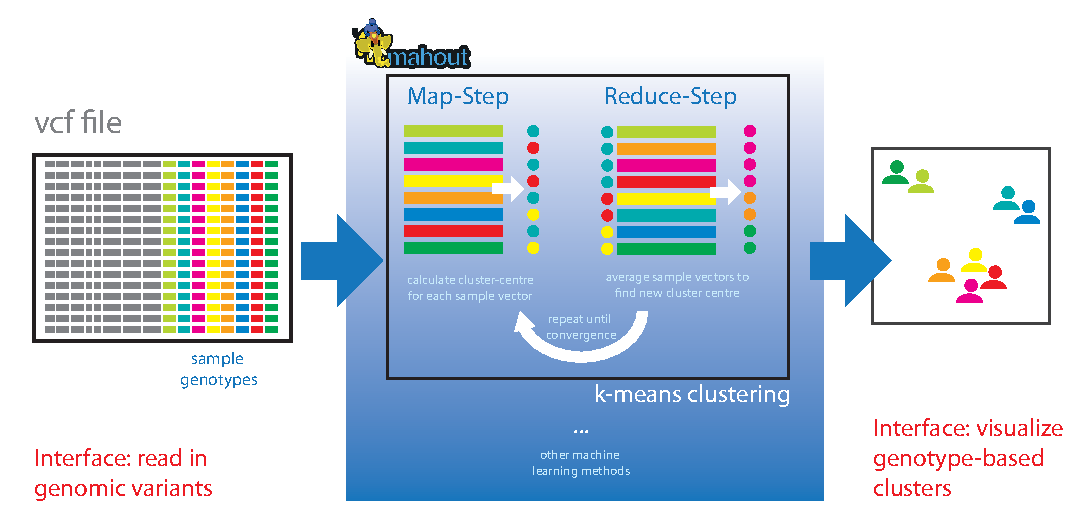
\includegraphics[type=pdf,ext=.pdf,read=.pdf, scale=0.40]{signature}}
        \label{fig:sign}
        \caption{{\bf Illustration of Mahout-based clustering of genotypes.}
      The image shows how the here introduced interface converts the VCF file to a mahout usable vector-based data type. Based on k-means it illustrates how the Map-step procedure groups of vectors by their nearest cluster center and the Reduce-step averages the vectors in each group to find the new value of the updated cluster center. The mahout-produced output is then converted into a visualisation.}

\end{figure}


\section{Key Points}
\begin{itemize}
\item Many bioinformatics tasks can be converted into the MapReduce-paradigm making Hadoop-based approaches attractive.
\item Scaling seamlessly to larger data sets has been celebrated as Hadoop's superior functionality over conventional parallelisation methodologies, however this only applies on resource-uncapped machines. 
\item On machines available in research settings, we demonstrate that achieving optimal performance still requires careful resource adjustment taking machine architecture and dataset features into account. 
\item Unlike R, Hadoop-based approaches make clustering of genome wide sequencing variants from cohorts with 2500 individuals feasible on machines available in research settings.
\end{itemize}


\section*{Acknowledgement}
A.R.O was funded by the NSW Cancer Institute Big Data Big Impact schema, F.A.B by the National Health and Medical Research Council [1051757] and both D.C.B and N.S by Commonwealth Scientific and Industrial Research Organisation's Transformational Capability Platform, Science and Industry Endowment Fund and Information Management and Technology Services. The computation on Azure was funded by Microsoft Azure Research Award. 
The authors would like to thank Piotr Szul and Gareth Williams for their help with setting up Hadoop on the HPC system.

%\bibliographystyle{natbib}
%\bibliographystyle{achemnat}
%\bibliographystyle{plainnat}
\bibliographystyle{abbrv}
%\bibliographystyle{bioinformatics}
\bibliography{genotypeClustering}  
\end{document}
